%% ++++++++++++++++++++++++++++++++++++++++++++++++++++++++++++
%% Hauptdatei, Wurzel des Dokuments
%% ++++++++++++++++++++++++++++++++++++++++++++++++++++++++++++
%
%

% Headerfeld, Typ des Dokumentes, einzubindende Packages.
% Hier bei Bedarf Änderungen vornehmen.
\documentclass
[   twoside=false,     % Einseitiger oder zweiseitiger Druck?
    fontsize=12pt,     % Bezug: 12-Punkt Schriftgröße
    DIV=15,            % Randaufteilung, siehe Dokumentation "KOMA"-Script
    BCOR=0mm,         % Bindekorrektur: Innen 17mm Platz lassen. Copyshop-getestet.
%    headsepline,
    headsepline,  % Unter Kopfzeile Trennlinie (aus: headnosepline)
    footsepline,  % Über Fußzeile Trennlinie (aus: footnosepline)
    open=right,        % Neue Kapitel im zweiseitigen Druck rechts beginnen lassen
    paper=a4,          % Seitenformat A4
    abstract=true,     % Abstract einbinden
    listof=totoc,      % Div. Verzeichnisse ins Inhaltsverzeichnis aufnehmen
    bibliography=totoc,% Literaturverzeichnis ins Inhaltsverzeichnis aufnehmen
    titlepage,         % Titelseite aktivieren
    headinclude=true,  % Seiten-Head in die Satzspiegelberechnung mit einbeziehen
    footinclude=false, % Seiten-Foot nicht in die Satzspiegelberechnung mit einbeziehen
    numbers=noenddot   % Gliederungsnummern ohne abschließenden Punkt darstellen
]   {scrreprt}         % Dokumentenstil: "Report" aus dem KOMA-Skript-Paket
	
\usepackage{etoolbox}
\usepackage[active]{srcltx}
%\usepackage[activate=normal]{pdfcprot} % Optischer Randausgleich -> pdflatex!
\usepackage{ifthen}
\usepackage[english]{babel}   % Neue Deutsche Rechtschreibung
%\usepackage[latin1]{inputenc} % Zeichencodierung nach ISO-8859-1
\usepackage[utf8]{inputenc}   %	Zeichencodierung nach UTF-8 (Unicode)
\usepackage[T1]{fontenc}
%\usepackage{ae} % obsolet und durch lmodern ersetzt
\usepackage{lmodern}
\usepackage[T1]{url}  
\usepackage[final]{graphicx}
\usepackage[automark]{scrpage2}
\usepackage{setspace}
%\usepackage[first,light]{draftcopy} % Für Probedruck
\usepackage[plainpages=false,pdfpagelabels,hypertexnames=false]{hyperref}
\usepackage{pdfpages}
\usepackage{array}
\usepackage{amssymb}
\usepackage{multirow}
\usepackage{hyperref}
\usepackage{breakurl}
\usepackage{booktabs}
\usepackage{fancyvrb}
\usepackage{amsmath}
\usepackage{setspace}
%\usepackage{times}
\usepackage{eurosym}


% Tiefe der Kapitelnummerierung beeinflussen
\setcounter{secnumdepth}{3} % Tiefe der Nummerierung
\setcounter{tocdepth}{3}    % Tiefe des Inhaltsverzeichnisses


% Hier in die zweite geschweifte Klammer jeweils
% die persönlichen Daten und das Thema der Arbeit eintragen:
\newcommand{\artderausarbeitung}{}
\newcommand{\namedesautors}{Wernecke, Luise, Student ID: 03645807}
\newcommand{\themaderarbeit}{Optimierung der Informationsverteilung für Car-2-X-Kommunikation}

% PDF Metadaten definieren
\hypersetup{
   pdftitle={\themaderarbeit},
   pdfsubject={\artderausarbeitung},
   pdfauthor={\namedesautors},
   pdfkeywords={\artderausarbeitung; TU-Ilmenau; Kommunikationsnetze;}}


% Abkürzungsverzeichnis beeinflussen. Hier nichts ändern!
\usepackage[intoc]{nomencl}
  \let\abbrev\nomenclature
  \renewcommand{\nomname}{Abkürzungsverzeichnis und Formelzeichen}
  \setlength{\nomlabelwidth}{.25\hsize}
  \renewcommand{\nomlabel}[1]{#1 \dotfill}
  \setlength{\nomitemsep}{-\parsep}
  \makenomenclature
\usepackage[normalem]{ulem}
  \newcommand{\markup}[1]{\textbf{#1}}

% Seitenlayout festlegen. Hier nichts ändern!
\pagestyle{scrplain}
\ihead[]{}
\ohead[]{}
\chead[]{}
\ifoot[]{ \pagemark}
\ofoot[]{\footnotesize  \namedesautors }
\cfoot[]{}
\textwidth = 159mm

\renewcommand{\titlepagestyle}{scrheadings}
\renewcommand{\partpagestyle}{scrheadings}
\renewcommand{\chapterpagestyle}{scrheadings}
\renewcommand{\indexpagestyle}{scrheadings}

% Abschnittsweise Nummerierung anstatt fortlaufend. Hier nichts ändern!
\makeatletter
\@addtoreset{equation}{chapter}
\@addtoreset{figure}{chapter}
\@addtoreset{table}{chapter}
%\renewcommand\theequation{\thechapter.\@arabic\c@equation}
%\renewcommand\thefigure{\thechapter.\@arabic\c@figure}
%\renewcommand\thetable{\thechapter.\@arabic\c@table}
%\makeatother

% Quelltextrahmen, klein. Hier nichts ändern!
\newsavebox{\inhaltkl}
\def\rahmenkl{\sbox{\inhaltkl}\bgroup\small\renewcommand{\baselinestretch}{1}\vbox\bgroup\hsize\textwidth}
\def\endrahmenkl{\par\vskip-\lastskip\egroup\egroup\fboxsep3mm%
\framebox[\textwidth][l]{\usebox{\inhaltkl}}}

% Quelltextrahmen, normale Groesse. Hier nichts ändern!
\newsavebox{\inhalt}
\def\rahmen{\sbox{\inhalt}\bgroup\renewcommand{\baselinestretch}{1}\vbox\bgroup\hsize\textwidth}
\def\endrahmen{\par\vskip-\lastskip\egroup\egroup\fboxsep3mm%
\framebox[\textwidth][l]{\usebox{\inhalt}}}

% Trennvorschläge für falsch getrennte Wörter.
% Wird häufig bei eingedeutschen Wörtern benötigt, da LaTeX hierbei
% gerne falsch trennt. Alternativ kann auch im Fliesstext ein
% Trennvorschlag per "\-" hinterlegt werden, bspw.:
% Die Hard\-ware besteht aus A und B.



% Sonstige Befehlsdefinitionen hier ablegen.
\newcommand{\entspricht}{\stackrel{\wedge}{=}}

\begin{document}
\onehalfspacing

\title{\LARGE Digital Signal Processing Laboratory \\  Project1: Time-Delay estimation in GNSS \\ Lab Report }
\author{\large Luise Wernecke \\  \large Student ID: 03645807\\ \large Master of Electrical and Information Engineering}
\date{\large 26.05.2014}

\maketitle


% Die einzelnen Kapitel
\begingroup
\let\clearpage\relax

\pagenumbering{arabic}
\pagestyle{scrheadings}
%% ++++++++++++++++++++++++++++++++++++++++++++++++++++++++++++
%% Kapitel 1: Einleitung
%% ++++++++++++++++++++++++++++++++++++++++++++++++++++++++++++


\chapter{Introduction}
In Global Navigation Satellite Systems (GNSS), including GPS, GNSS and GLONASS, the first step for the receiver is scanning all satellites insight. This process is called aquisition. Every satellite continuously transmit a signal contain the special Pseudo Random Code (PRN) belonging to satellite. By decoding this signal the receiver knows from which satellite the signal comes from. All possible PRN codes are stored in the receiver. One of the characteristic of the PRN is that they are completely orthogonal. Consequently, the correlation between the code and the received signal has if and only if a peak if it is exactly the same code. Because the code received within the signal can be time-shifted, this delay $\tau$ has to be searched to verify the satellite ID. 

There are two possible search strategies to get $ \tau $. The first method is a sequential search, where correlations for each $\tau$ are calculated and looked for a peak. If it is the wrong code only noise occur. For this I created a for-loop with an amount of different $\tau$ in steps of $ 1 / f_{s} =  977.52 \mu s$ corresponding to one chip. For each shifted code the correlation will be calculated with $ C = \mid(y^{T}\cdot c(\tau )\mid $ with $y^{T}$ being the transposed received signal and $c(\tau )$ the code signal shifted by $\tau$. Afterwards, the maximum correlation will be calculated, which corresponds to the searched $\tau$.

\begin{figure}[!ht]
\centering
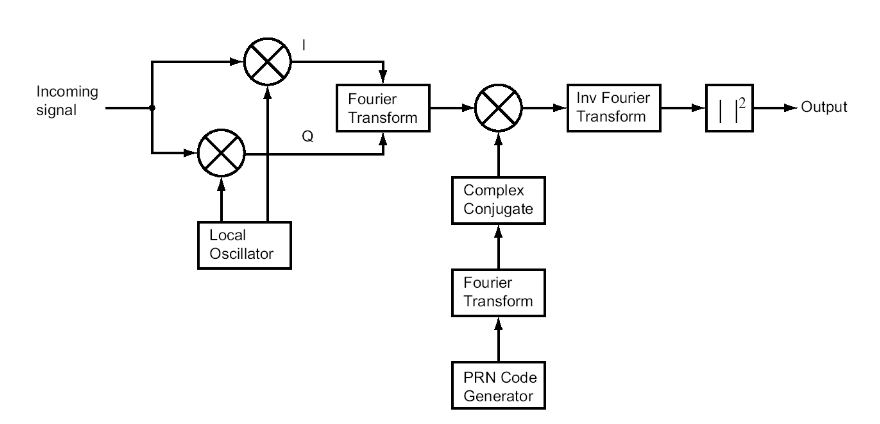
\includegraphics[scale=0.5]{bilder/method.png} 
\caption{Parallel Code Phase Search}
\label{bild:method}
\end{figure}

Another more time-efficient method is a parallel code phase search corresponding to \ref{bild:method}. This method uses the fast fourier transformation to search only for one loop. A correlation can be expressed like this formulation:

\[ C\left[ n = \triangle \tau \right] = y \left[ n \right] \bigotimes c \left[ \tau \right]  =  \sum \limits_{m=0}^{N-1}y\left[ m \right] \bigotimes c \left[n + m \right] \] 

After fourier transformation both signals can be multiplied:

\[C \left[ k \right]  =  Y\left[ k \right]  \cdot C^{ \ast } \left[ k \right]   \] 

and back transformed it corresponds to the correlation again.

\[C \left[ n \right]^{2}  =  F_{FFT}^{-1} \left\lbrace Y\left[ k \right]  \cdot C^{ \ast } \left[ k \right] \right\rbrace  ^{2}  \] 

By implementing this only the code with $ \tau $ = 0 has to be generated and transformed into the fourier domain as well as the received signal. Afterwards, the received signal with the conjugated complex code signal will be multiplied and back transformed.  Due to the calculation in frequency domain all different time-shifted correlations are calculated. The property of fourier transformation is exactly this time-shifting. After back-transformation you can see a plot of $ C\left[ m \right]  $ like \ref{bild:corr}. At the point of the peak is the searched $ \tau $. It is 400 $ T_{c} $ long. 

By comparing both methods the sequential search takes about 8 s while the parallel search only takes 50 ms. Therefore, the second method is much faster and thus more suitable. The restriction for the time, there, is only the algorithm of the fast fourier transform, which could be for example a Decimation-in-Frequency or Decimation-in-Time algorithm.

\begin{figure}[!ht]
\centering
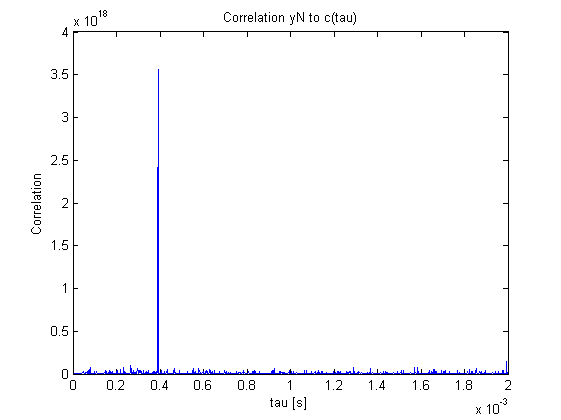
\includegraphics[scale=0.5]{bilder/results.png} 
\caption{Correlation over different $ \tau $}
\label{bild:corr}
\end{figure}


\newpage
%% Literaturverzeichnis einbinden
%%% ++++++++++++++++++++++++++++++++++++++++++++++++++++++++++++
%% Anhang: Literaturverzeichnis
%% ++++++++++++++++++++++++++++++++++++++++++++++++++++++++++++
%
%  Gerüst:
%  * Version 0.11
%  * Dipl.-Ing. Karsten Renhak, karsten.renhak@tu-ilmenau.de
%  * Fachgebiet Kommunikationsnetze, TU Ilmenau
%
%  Für Hauptseminare, Studienarbeiten, Diplomarbeiten
%
%  Autor           : Max Mustermann
%  Letzte Änderung : 31.12.2011
%

% Mit dem Befehl \nocite werden auch nicht im Text zitierte
% aus der Literaturdatenbank mit in das Literaturverzeichnis aufgenommen.
% Ein "\nocite{*}" übernimmt ungeprüft die komplette Datenbank.
%\nocite{*}

\cleardoublepage
\ihead[]{Literaturverzeichnis}
\bibliographystyle{alphadin}
\bibliography{literatur} % "literatur.bib" ist hier die einzige Literaturdatenbank.

% Alternativ: Mehrere Datenbanken verwenden, falls eine
% oder mehrere umfangreiche Sammlungen exisitieren:
%\bibliography{literatur_buecher,literatur_weblinks}

%
%% Abbildungsverzeichnis einbinden
%%% ++++++++++++++++++++++++++++++++++++++++++++++++++++++++++++
%% Anhang: Abbildungsverzeichnis
%% ++++++++++++++++++++++++++++++++++++++++++++++++++++++++++++
%
%  Gerüst:
%  * Version 0.11
%  * Dipl.-Ing. Karsten Renhak, karsten.renhak@tu-ilmenau.de
%  * Fachgebiet Kommunikationsnetze, TU Ilmenau
%
%  Für Hauptseminare, Studienarbeiten, Diplomarbeiten
%
%  Autor           : Max Mustermann
%  Letzte Änderung : 31.12.2011
%

% Keine Änderungen vornehmen!
\cleardoublepage
\ihead[]{Abbildungsverzeichnis}
\listoffigures



\endgroup
\end{document}

